\documentclass{fkssolpub}

\usepackage[czech]{babel}
\usepackage{fontspec}
\usepackage{fkssugar}
\usepackage{amsmath}
\usepackage{graphicx}
\usepackage{caption}

\author{Ondřej Sedláček}
\school{Gymnázium Oty Pavla} 
\series{2p}
\problem{5} 

\begin{document} 

Jako první si ukážeme, jak najít $2n - 1$ provincií, které se do sebe vejdou. Jako
první si sloupce a řádky ve čtverci seřadíme podle jejich velikosti tak, že nahoře
bude nejvyšší řádek a vlevu bude nejširší sloupec. Pak si vybereme $2n - 1$ provincií
tak, jako je znázorněno tmavými políčky na obrázku níže. Protože pro každý pár provincií 
ve vybrané
množině platí, že buď jednou hranou sousedí, nebo jedna z nich má oba rozměry menší než 
druhá provincie, stačí nám už ukázat, že vždy najdeme ještě jednu další provincii tak,
abychom splnili zadání.

Nechť jsou šířky sloupců $a_1 \geq a_2 \geq ... \geq a_n$ a výšky řádků $b_1 \geq b_2
\geq ... \geq b_n$. Budu sporem dokazovat, že můžeme vybrat alespoň jeden ze světle šedých 
provincií tak, abychom splnili zadání.
Zřejmě není zaručeno, že se provincie do sebe vejdou bez otočení. Zároveň
víme, že jedna ze světle šedě zvýrazněných provincií o rozměřech $(a_{i+1}, b_i)$ se
vejde do všech provinií množiny kromě provincie o rozměrech $(a_i, b_{i + 1})$ (o ní nevíme,
jestli se vejdou do sebe).
Aby se provincie s rozměry $(a_{i+1}, b_i)$ a $(a_i, b_{i + 1})$ po otočení vešli do sebe, 
musí platit výrok:

\[
  (\exists i \in \{1, 2, ..., n - 1\}) (a_i \geq b_i \Leftrightarrow b_{i + 1} \geq a_{i + 1})
\]

Předpokládejme, že se do této provincie nevejde, tudíž, že platí jeho negace:

\[
  (\forall i \in \{1, 2, ..., n - 1\}) (a_i \geq b_i \Leftrightarrow a_{i + 1} > b_{i + 1})
\]

Pokud tato negace platí, musí platit:

\[
  \left(\sum_{i=0}^{n} a_i > \sum_{i=0}^{n} b_i \right) \qquad \lor \qquad \left( \sum_{i=0}^{n} a_i < \sum_{i=0}^{n} b_i \right)
\]

PraSestán má však tvar čtverce, tudíž jsme došli ke sporu a tedy jsme vždycky schopni
najít $2n$ provincií, které se do sebe vejdou. Q. E. D.

\begin{figure}[h!]
  \centering
  \captionsetup{justification=centering,margin=2cm}
  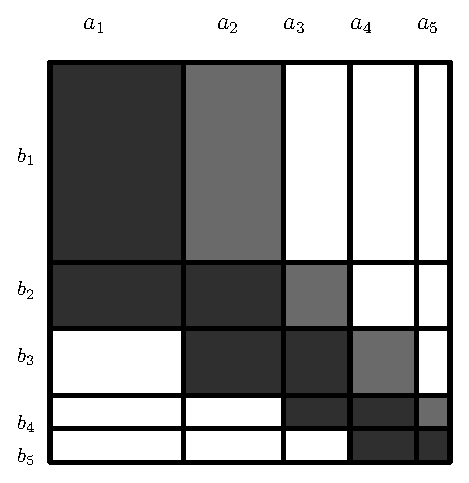
\includegraphics{5-fig}
  \caption{Názorné schéma pro PraSestán o $n = 5$. \\ Tmavé se jistě vejdou do sebe,
  u světlých alespoň jedna z nich.}
\end{figure}

\end{document}
